\chapter{KD-Trees}\label{chp:kdTrees}

%% \chapterquote{In theory, there is no difference between theory and
%%   practice. But, in practice, there is.}{Jan L. A. van de Snepscheut}

\chapterquote{With todays's fast ray tracers, the difference between a
  ``good'' and a naïvely built kd-tree is often a factor of 2 or
  more.}{Ingo Wald and Vlastimil Havran}

% About KD-trees

Before we in \refchapter{chp:rayTracing} discuss how the rays will
traverse the hierarchical acceleration structure, we must first
examine that structure.

% Why KD tree compared to other structures

As mentioned earlier in this thesis, kd-trees was chosen as the data
structure employed to accelerate ray tracing. This choice is based on
several factors.

% Cheap intersection / distance to tests. Havran p. 51

One of them is the ease with which the signed distance from a ray to a
kd-trees axis aligned splitting plane can be computed. The splitting
plane can be described by an axis, $d \in \{x, y, z\}$, and it's
position along that axis, $N_d$. The signed distance from any ray,
$R(t) = O + tD$, to the splitting plane is then simply calculated as

\begin{displaymath}
  t = \frac{N_d - O_d}{D_d}
\end{displaymath}

For comparison a generel \textit{binary space partition} tree,
\textit{BSP} tree, with arbitrarily oriented splitting planes, given
by $ax + by + cz + d = 0$ has a much more complex distance function.

\begin{displaymath}
  t = \frac{a O_x + b O_y + c O_z + d}{a D_x + b D_y + c D_z}
\end{displaymath}

It becomes even more complex when bounding volumes are used. An axis
aligned bounding box can be described by 2 points, $V_{min}$ and
$V_{max}$. Calculating the signed distance to any rays entry and exit
point is then

\begin{displaymath}
  \begin{array}{l}
    t_{near,d} = min((V_{min,d} - O_d) / D_d, (V_{max,d} - O_d) / D_d)\\
    t_{entry} = max(t_{near,x}, t_{near,y}, t_{near,z})
  \end{array}
\end{displaymath}

The distance from the ray origin to all of the bounding box sides are
calculated, then the minimum along each axis is chosen and the maximum
of these values are the distance to the entry point. The distance to
the exit point is calculated similarly.

\begin{displaymath}
  \begin{array}{l}
    t_{far,d} = max((V_{min,d} - O_d) / D_d, (V_{max,d} - O_d) / D_d)\\
    t_{exit} = min(t_{far,x}, t_{far,y}, t_{far,z})
  \end{array}
\end{displaymath}


If the rays exit distance lies closer than the entry distance, then
the ray did not intersect the bounding volume, an example of this is
given on \reffig{fig:rayBoxIntersection}.

\begin{figure}
  \centering
%  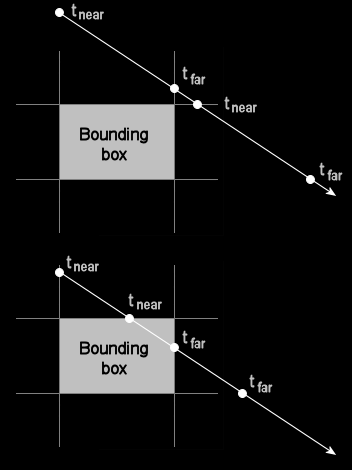
\includegraphics[width=5cm]{RayBoxIntersection}
  \subfloat[Ray miss.]{
    \begin{tikzpicture}[y=0.5cm, x=.5cm,font=\sffamily]
      % Planes
      \draw[dashed, color=gray] (-2,0) -- (5,0);
      \draw[dashed, color=gray] (-2,2) -- (5,2);
      \draw[dashed, color=gray] (0,3.5) -- (0,-1.5);
      \draw[dashed, color=gray] (3,3.5) -- (3,-1.5);

      % AABB
      \draw (0,0) -- (3,0) -- (3,2) -- (0,2) -- (0,0);

      % Ray
      \drawRay{0,5}{8,-1}

      % Intersection
      \draw[fill=black] (0,5) circle (0.05cm);
      \draw (1,5.3) node{$t_{near,y}$};
      \draw[fill=black] (3,2.75) circle (0.05cm);
      \draw (4,3.05) node{$t_{far,y}$};
      \draw[fill=black] (4,2) circle (0.05cm);
      \draw (5,2.3) node{$t_{near,x}$};
      \draw[fill=black] (6.66,0) circle (0.05cm);
      \draw (7.66,0.3) node{$t_{far,x}$};

    \end{tikzpicture}
  }
  \subfloat[Ray hit.]{
    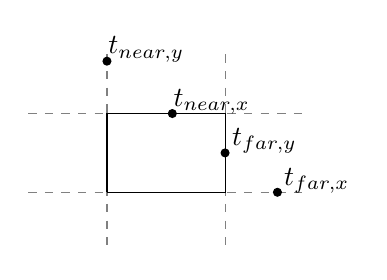
\begin{tikzpicture}[y=0.5cm, x=.5cm,font=\sffamily]
      % Planes
      \draw[dashed, color=gray] (-2,0) -- (5,0);
      \draw[dashed, color=gray] (-2,2) -- (5,2);
      \draw[dashed, color=gray] (0,3.5) -- (0,-1.5);
      \draw[dashed, color=gray] (3,3.5) -- (3,-1.5);

      % AABB
      \draw (0,0) -- (3,0) -- (3,2) -- (0,2) -- (0,0);

      % Ray
      \drawRay{-1,4}{7,-2}

      % Intersection
      \draw[fill=black] (0,3.33) circle (0.05cm);
      \draw (1,3.63) node{$t_{near,y}$};
      \draw[fill=black] (1.66,2) circle (0.05cm);
      \draw (2.66,2.3) node{$t_{near,x}$};
      \draw[fill=black] (3,1) circle (0.05cm);
      \draw (4,1.3) node{$t_{far,y}$};
      \draw[fill=black] (4.33,0) circle (0.05cm);
      \draw (5.33,0.3) node{$t_{far,x}$};

    \end{tikzpicture}
  }
  \caption{Ray/Box intersection.}
  \label{fig:rayBoxIntersection}
\end{figure}

Clearly kd-trees provide the simplest distance calculations of the
above given examples.

% Example of kd-tree flexibility over octree (important in sparse
% scenes / empty space partitioning)

Binary trees, such as kd- and bsp trees, are also more flexible than
quadtress or octrees. An example can be seen on
\reffig{fig:binQuadSplit}. This flexibility can be extremely important
when accelerating sparse scenes.

\begin{figure}
  \centering
  \subfloat[Possible binary splits.]{
    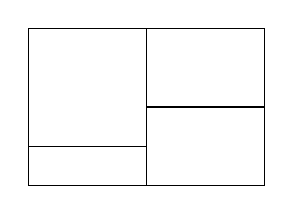
\begin{tikzpicture}[y=0.5cm, x=.5cm,font=\sffamily]
      
      % AABB
      \draw (0,0) -- (6,0) -- (6,4) -- (0,4) -- (0,0);
      
      % TRIS
      \drawTri{0,4}{3,3}{1.5,1}
      \drawTri{6,1}{4, 2}{4,0}
      
      % splits
      \draw (3,0) -- (3,4);
      \draw (0,1) -- (3,1);
      \draw (3,2) -- (6,2);
      
    \end{tikzpicture}
    \label{fig:binarySplit}
  }
  \hspace{20pt}
  \subfloat[Possible quadternary splits.]{
    \begin{tikzpicture}[y=0.5cm, x=.5cm,font=\sffamily]
      
      % AABB
      \draw (0,0) -- (6,0) -- (6,4) -- (0,4) -- (0,0);
      
      % TRIS
      \drawTri{0,4}{3,3}{1.5,1}
      \drawTri{6,1}{4, 2}{4,0}
      
      % splits
      \draw (3,0) -- (3,4);
      \draw (0,1) -- (6,1);
      
    \end{tikzpicture}
    \label{fig:quadternarySplit}
  }

  \parbox{9cm}{\caption[Comparisson of binary and quadternary
      splitting]{A comparisson of binary and quadternary
      splitting. Notice that the binary splitting planes can be placed
      without intersecting any geometry.}\label{fig:binQuadSplit}}
\end{figure}

% Vlastimil Havran did an extensive study of available spatial
% subdivision schemes (including regular grids, nested grids, octrees
% and kd-trees) and concludes in his phd thesis that kd-trees are
% better than the other schemes in most cases.

Finally, in his phd. dissertation, Vlastimil Havran did an extensive
study of spatial data structures, including grids, octress and
kd-trees, and found that the kd-tree performed the best in most cases.

Given all of the above and with the recent paper by \zhou{}, in which
kd-trees are constructed in real-time on graphics hardware, it is easy
to see why the choice fell on kd-trees as the acceleration structure.

% About this Chapter. Start by motivation. Then explain how kd-trees
% are constructed, including different strategies for choosing the
% spliting plane and doing the actual geometry splitting. Then the
% chapter will end with a discussion of how to implement the
% algorithms efficiently on a SIMT architecture.

In the rest of this chapter, we will first examine how kd-trees are
built. In particular different algorithms for choosing the splitting
plane candidate will be studied and how to handle geometry
intersecting the splitting plane will be discussed. The latter part of
this chapter deals with converting a sequential kd-tree construction
algorithm into a dataparallel algorithm. Focus is split between upper
tree nodes and lower tree nodes, once the number of geometric
primitives per node goes below a certain threshold.

\section{Building KD-trees}

A kd-tree is a binary tree that recursively subdivides geometry into
smaller tree nodes. \refalg{alg:kdTreeCreator} describes a generel
recursive kd-tree construction scheme.

\begin{algorithm}
  \caption{Recursive kd-tree constructor}
  \label{alg:kdTreeCreator}
  \begin{algorithmic}
    \PROCEDURE{ConstructKDTree}
              {$T$ : Triangle List; $voxel$ : AABB}
              {$node$ : KDNode}
              {\IF{IsLeaf($T, voxel$)}
                  \ASSIGN{$node$}{Leaf(T)}
                \ELSE
                  \COMMENTIT{Determining the splitting plane will be discussed in \refsection{sec:splittingPlane}}
                  \ASSIGN{$plane$}{DeterminePlane($T, voxel$)}
                  \ASSIGN{$(voxel_L, voxel_R)$}{Split($voxel, p$)}
                  \COMMENTIT{How to associate geometry with a voxel will be the topic of  \refsection{sec:splittingGeom}}
                  \ASSIGN{$T_L$}{AssociateGeometry($T, voxel_L$)}
                  \ASSIGN{$T_R$}{AssociateGeometry($T, voxel_R$)}
                  \ASSIGN{$node$}{Node($plane$, ConstructKDTree($T_L, voxel_L$), ConstructKDTree($T_R, voxel_R$))}
                \ENDIF}
  \end{algorithmic}
\end{algorithm}

ConstructKDTree takes as arguments a list of triangles and an axis
aligned bounding box defining the volume of the node. The algorithm
then checks if the triangles and bounding box satisfy the requirements
of beeing a leaf node. If so, then a leaf is produced and the
recursion terminates. If not then a splitting plane, $plane$, needs to
be determined and the bounding box is divided by $plane$, producing a
new left and right axis aligned bounding box. Triangles are then
distributed to each new bounding box by some decision algorithm and a
new node is created that will contain references to it's 2 children.

\fixme{mention bounding box recomputing, probably not in this generel
  case.}

% Left balanced non pointer vs pointers

In generel there are 2 ways a node can reference its child nodes. The
first is \textit{balanced trees}, where children of a node can be
addressed implicitly without the use of pointers. The reason for this
is that nodes at the same tree level are placed sequantially in
memory. The left and right child of node $n$ can then be indexed using
$2n+1$ and $2n+2$. The parent of a node is indexed with $\lceil n/2
\rceil - 1$.

% Balanced trees suck, example of partition with high density in one
% side and no triangles in other side. 

Wald et al.\citebook{wald:04:VVH} has the following to say about
balanced trees.

\quotebook{Balancing is optimal only for binary searching, and if all
  nodes have equal access probabilities. Neither of these two
  prerequisites are fulfilled for range queries (such as ray traversal
  and kNN queries), nor for unevenly distributed primitives such as
  photons or triangles.}{wald:04:VVH}

% Choose pointers as that would lead to less memory consumption and it
% places all nodes of the same level in a continues block, making it
% easier to work with them.

To avoid balanced trees we can instead use pointers to reference the
children. This allows for more flexibility when creating the tree.
Unfortunatly it also means storing more data per node and in the case
of slow memory access it could cause a memory latency
bottleneck. However, in a survay of different techniques such as this
thesis, the added flexibility can be a benefit and in
\refsection{sec:gpuEmptySpace} we shall see how this flexibility can
be used to add empty space splitting, something that could not have
been done as unobtrusive had the tree been balanced.




\subsection{Choosing the Splitting Plane}\label{sec:splittingPlane}

% All the brilliance in KD-tree construction comes down to choosing
% the splitting plane and deciding when to stop.

Looking again at \refalg{alg:kdTreeCreator}, we can see that all the
brilliance in constructing a high quality kd-tree is knowing where to
place the splitting plane and when to end the recursion and create a
leaf.

% Different splitting planes heuristics.

In the following section 2 algorithms that solves this problem is
presented and then extended with empty space splitting.


\subsubsection{Spatial Median}

% Split at the spatial median.

% Axis to split along can be choosen in a round robin fashion or the
% largest axis can be choosen. (Which initially minimises the surface
% of the children)

A quite simple method of choosing the splitting plane is to place it
at the spatial median of the nodes bounding box. There are 2 ways to
choose which dimensional spatial median to use. A \textit{round robin}
fashion can be used, where the dimensions are cycled every iteration;
ie. when creating the first node the plane will lie perpendicular to
the x-axis, the children will then be split along the y-axis, in the
next iteration the plane will split along the z-axis and then restart
again at x. Another way of choosing the dimension is to split along
the largest axis of the node's bounding box. This can be more costly
than the round robin approach, since the entire bounding box will have
to be calculated each iteration, but it will also produce the best
results.

The termination requirement for spatial median splitting is equally as
simple as choosing the splitting plane. If the number of triangles per
node falls below a certain threshold, iteration stops.

% Refered to as the naïve implementation in Wald07.

This method is refered to as naïve in \citebook{wald:06:NlogN} and
rightly so. Not much thought is put into the distribution of geometry
inside the bounding box. On \reffig{fig:crapMedian} an example is
given where the node is split in a non-intuitive way. Spatial median
splitting does, however, make up for its suboptimal splitting planes
by being quite fast, and I will therefore use it for creating my
kd-trees upper nodes, as is described in \refsection{sec:upperNodes}.

\begin{figure}
  \centering
  \begin{tikzpicture}[y=0.5cm, x=.5cm,font=\sffamily]
    % AABB
    \draw (0,0) -- (6,0) -- (6,4) -- (0,4) -- (0,0);

    % Tris
    \drawTri{0,0}{2,4}{4,0}
    \drawTri{5,4}{5.5,4}{5,3}
    \drawTri{5,2.5}{5.5,2.5}{5.5,3.5}
    \drawTri{5,2}{6,2}{5.5,0.5}

    % Split
    \draw (3,0) -- (3,4);
    \draw[dashed] (5,0) -- (5,4);

  \end{tikzpicture}

  \vspace{3mm}
  \parbox{5cm}{\caption[A poor split produced by median splitting.]{A
      poor split produced by median splitting. The solid line is a
      median split. The dashed one is a more optimal splitting plane,
      since it divides the large triangle from the
      small.}\label{fig:crapMedian}}
\end{figure}

\subsubsection{Surface Area Heuristic}

% SAH assumptions can be seen in Wald07

A far better splitting plane position can be obtained by applying the
\textit{surface area heuristic}, \textit{SAH}. Instead of only
considering the bounding volume surrounding the geometry, SAH
considers the entire geometry of a node. In essence SAH computes the
\textit{expected cost} of traversing a node, $N$, with child nodes $L$
and $R$.

\begin{displaymath}
  SAH(N \rightarrow \{L, R\}) = C_N + \frac{C_L A_L}{A_N} +
  \frac{C_R A_R}{A_N}
\end{displaymath}

where $C_N$ is the cost of traversing the node itself and is
independent of the splitting plane, $C_L$ is the cost of traversing
the left child node and $C_R$ is the cost of traversing the right
child node. $A_n$ is the summed surface area of all primitives in node
$n$. Choosing the best splitting plane amounts to applying SAH to all
possible splitting planes and then choosing the one with lowest
cost. Since the above cost evaluation does not take rays into account,
SAH assumes that rays are uniformly distributed, infinite lines.

SAH can also automatically determine when to stop splitting. Assuming
that the cost of intersecting a leaf is given as $C_{leaf} = |T| *
C_i$, where $|T|$ is the number of triangles and $C_i$ is the cost of
intersecting a triangle. SAH's termination criteria is then $C_{leaf}
< C_N$, i.e. SAH terminates when the cost of intersecting a leaf
becomes less than the cost of most optimal splitting plane.

% Globlly optimal is infeasable for complex scenes and instead a local
% greedy approximation is used.

Calculating a globally optimal solution using SAH is infeasable,
except for trivially simple scenes. A \textit{local greedy
  approximation} is used instead, where it is assumed that the created
child nodes are leafs.

Inspite of all the assumptions made by SAH, which in practice do not
hold, it is still considered one of the best heuristics and produces
trees of the highest quality.

% SAH calculation optimizations include axis round robin and some damn
% paper I can't remember.


\paragraph{Split Candidates}

% To avoid having to test the infinitely many splitting planes
% possible, we instead have to choose sensible planes for SAH.

As mentioned above the SAH cost needs to be calculated for
\textit{all} available splitting planes. Since there infinitely many
potential planes along either axis, we need some method to distinguish
useful split candidates from unimportant ones. That means we're only
interested in those finitely many planes where the geometry
association in the resulting left and right child nodes change.

% Take planes from bounding volumes

The obvious choice is to use the 6 planes defined by the triangles
axis aligned bounding box. While this is a simple and fast solution,
it can create a bloated tree, since triangles do not necessarily
overlap a node's bounding box, simply because its own bounding box
does. An example can be seen on \reffig{fig:aabbSplit}

\begin{figure}
  \centering
  \begin{tikzpicture}[y=0.5cm, x=.5cm,font=\sffamily]

    % AABB
    \draw (0,0) -- (5,0) -- (5,4) -- (0,4) -- (0,0);

    \drawTri{3,6}{7,2}{6,5}
    \drawAabb{3,2}{7,2}{7,6}{3,6}

  \end{tikzpicture}

  \vspace{3mm}
  \parbox{5cm}{\caption[Triangle/Node bounding box intersection.]{An
      example of how a triangles bounding box, the dashed box, can
      overlap a nodes bounding box, while the triangle itself does
      not.}\label{fig:aabbSplit}}
\end{figure}

Another problem with this approach is that bounding boxes of small
nodes may be completely contained inside the geometry's bounding box
and thus none of the planes are actually useful split
candidates. \reffig{fig:aabbContained} demonstrates this.

\begin{figure}
  \centering
  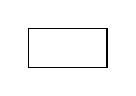
\begin{tikzpicture}[y=0.5cm, x=.5cm,font=\sffamily]

    \drawTri{0,4}{4,0}{3,3}
    \drawAabb{0,0}{4,0}{4,4}{0,4}

    % AABB
    \draw (1,1) -- (3,1) -- (3,2) -- (1,2) -- (1,1);

  \end{tikzpicture}
    
  \vspace{3mm}
  \parbox{5cm}{\caption[A tree node's bounding box contained in a
      triangle's bounding box.]{The kd-tree node's bounding box
      completely contained inside the triangles bounding
      box.}\label{fig:aabbContained}}
\end{figure}

A solution is to continuously \textit{clip} the bounding box of the
split geometry to fit the part of the geometry inside the tree nodes
bounding box, creating \textit{perfect split} condidates, as
demonstrated on \reffig{fig:aabbClipped}.

\begin{figure}
  \centering
  \begin{tikzpicture}[y=0.5cm, x=.5cm,font=\sffamily]

    \drawTri{0,4}{4,0}{3,3}
    \drawAabb{0,2}{2,2}{2,4}{0,4}
    \drawAabb{2,0}{4,0}{4,3.3}{2,3.3}

    % AABB
    \drawNode{-1,0}{2,0}{2,5}{-1,5}
    \drawNode{2,0}{5,0}{5,5}{2,5}

  \end{tikzpicture}

  \vspace{3mm}
  \parbox{5cm}{ \caption[Triangle clipping.]{The triangles bounding
      box has been clipped to fit the part of the triangle contained
      in the nodes bounding boxes.}\label{fig:aabbClipped}}
\end{figure}

Another solution is to simply remove the offending triangles, reafter
refered to as \textit{false primitives}, from the node. This can be
done by performing a triangle/box intersection check, a derivation of
the \textit{seperating axis theorem}, as described by Möller in
\citebook{Moller:2005}.


\subsubsection{Empty Space Splitting}

An effective optimization to kd-trees is \textit{empty space
  maximization} or empty space splitting. The idea behind the
optimization is to cut away large empty parts of the scene, by placing
empty leaf nodes in the upper parts of the tree. This will provide the
rays with an early out option, skipping a large portion of the
geometry. An example can be seen in \reffig{fig:emptySpaceExample},
where the gray shaded node has been created as an empty space node,
allowing the ray to skip over the triangles above.

\begin{figure}
  \centering
  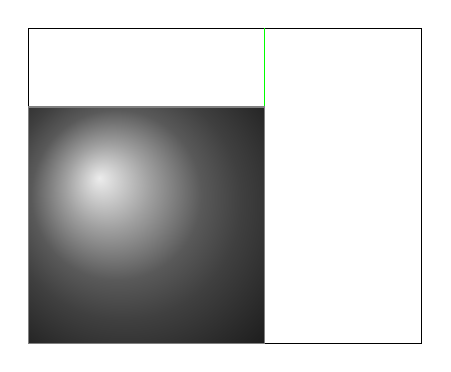
\begin{tikzpicture}[y=0.5cm, x=.5cm,font=\sffamily]

    % AABB
    \draw (0,0) -- (10,0) -- (10,8) -- (0,8) -- (0,0);

    % Tris
    \drawTri{9,0}{10,2}{6,3}
    \drawTri{7,8}{7,4}{9,4}

    \drawTri{0,8}{0,6}{2,8}
    \drawTri{1,7}{0,6}{2,6}
    \drawTri{1,7}{3,6}{3,8}
    \drawTri{5,7}{3,6}{3,8}
    \drawTri{5,7}{3,6}{6,6}

    % Splits
    \draw[color=green] (6,0) -- (6,8);
    \draw[color=green] (0,6) -- (6,6);

    % Empty space
    \draw[ball color=gray, color=green, shading=ball,gray] (0,0) -- (0,6) -- (6,6) -- (6,0) -- (0,0);

    % Ray
    \drawRay{0,0}{6,4}

  \end{tikzpicture}

  \vspace{3mm}
  \parbox{6cm}{\caption[Empty Space Splitting.]{An example of empty
      space splitting. The grey ball shaded area represents an empty
      node and allows the ray to leap across it and skip intersection
      tests with the 5 triangles above.}\label{fig:emptySpaceExample}}
\end{figure}


Unfortunatly, how large a percentage of a node that should be empty
before empty space splitting can cut it away is highly scene specific,
making this optimization less usefull in the general case. Like \zhou{}
I have found that performing an empty space split is optimal when a
bounding box is more than 25\% empty along one of the axes.

% Dynamic empty space threshold, favor early out in the top of the tree.

% huge ray tracing performance improvement in testscene (23% without
% raytracers doing intersection tests at leaf nodes)

% Implementation is 

\subsection{Splitting Schemes}\label{sec:splittingGeom}

This section will look at alternatives to triangle splitting, namely
\textit{triangle division}, where the triangle is not split by
splitting planes, but divided onto each side, by simply adjusting it's
bounding box, and \textit{box inclusion}, where the triangles
themselves are not tested for inclusion, but their bounding boxes are.

% What to do with the triangles caught in the splitting plane.



\subsubsection{Triangle splitting}

% Normally ppl split.

\subsubsection{Triangle dividing}

% Spliting will almost always produce 3 triangles, whereas divide will
% always produce only 2.

% Adjusting area heuristic: When we no longer split geometry, SAH
% becomes an even worse approximation. This can be fixed by an
% adjusting area heuristic, where the diagonal of the geometric
% primitives original bounding box is compared to the diagonal of the
% reduced box and the primitives surface area is adjusted accordingly.


\subsubsection{Box Inclusion}

% Simpler than splitting.

% Inspired by the small node step in Zhou

% Naturally increases amount of \textit{false primitives} in the tree, but is
% very cheap.

% Also has an increased change of looping during construction in
% combination with a small max lower size. Fx fairy forest loops using
% adjusting bounding box with a max size of 32 primtives in leaf nodes.

% False primitives can then be removed at a later stage at the cost of
% some extra overhead. Or combine with Divide every n'th step for
% optimal sweetness.

% With the added leaf intersection in the raytracer, extra triangles
% in the leaf nodes become even less important and this method starts
% to shine for dynamic scenes.






\section{Adopting the algorithms for GPGPUs}

% Needs to exploit the dataparallel nature of GPGPU's

% A GPGPU needs as many of its multiprocessors occupied as possibly
% for optimal performance.

% Use GPU for computations and let CPU handle minor book keeping.

% Handles structures of arrays better than arrays of structures
% chapter 33 \citebook{GPUGEMS2} and coalescence

\subsection{Upper Tree Nodes}\label{sec:upperNodes}

% At upper tree level nodes exploit data parallelism by parallising
% the cost computation over triangles. 

% SAH assumes that each split results in 2 leaf nodes, which is
% practically always wrong at high level nodes, therefore
% \citebook{1409079} suggests splitting along the spatial median of the
% nodes longest axis. To do this a preprocess pass is required to
% compute tight AABB's for each triangle.

% Creating the KD-tree in BFS will optimize GPU performance at lower
% tree levels, as there would be thousands of nodes created at the
% same time.

\begin{algorithm}
  \caption{KD-Tree upper node creator}
  \label{alg:kdUpperNodeCreator}
  \begin{algorithmic}
    \PROCEDURE{CreateUpperNodes}
               {\VAR{activeList}:list \textit{\color{gray}//list of kd-nodes not processed yet}}
               {\VAR{leafList,nextList}:list}{

                 \COMMENTIT{First split all triangles into segments.}
                 \DECLARE{$segmentList$}{list}
                 \PARALLELFOR{node \VAR{i} \textbf{in} activeList}
                   \STATE{Split all triangles contained in node $i$
                     into fixed sized segments and those in
                     $segmentList$.}
                 \ENDFOR
                 \STATE{}
                 \COMMENTIT{Then compute each triangles bounding box
                   using reduction as described in
                   \refsection{sec:reduce}.}
                 \PARALLELFOR{segment \VAR{s} \textbf{in} segmentList}
                   \STATE{Reduce the individual segments.}
                 \ENDFOR
                 \STATE{Using segmented reduction as described in
                   \zhou{}, reduce each nodes bounding box. Perform 
                   median splitting on the nodes.}

                 \STATE{}
                 \COMMENTIT{Perform Empty Space Splitting.}
                 \COMMENTIT{See \refalg{alg:emptySpaceSplitting}.}
                 \STATE{...}
                 \STATE{}

                 \COMMENTIT{Compute the addresses to move the triangles to.}
                 \DECLARE{$splitSide, splitAddr$}{list}
                 \PARALLELFOR{segment \VAR{s} \textbf{in} segmentList}
                   \ASSIGN{$triangles$}{$s$.triangles}
                   \PARALLELFOR{triangle \VAR{t} \textbf{in} triangles}
                   \STATE{Associate each triangle to its owner nodes
                     children, with respect the owner node's splitting
                     plane. Store the information in $splitSide$.}
                   \ENDFOR
                 \ENDFOR
                 \STATE{Using Scan compute the prefix-sum of
                   $splitSide$ and store it in $splitAddr$.}

                 \STATE{}

                 \COMMENTIT{Split the triangles.}
                 \PARALLELFOR{segment \VAR{s} \textbf{in} segmentList}
                   \ASSIGN{$triangles$}{$s$.triangles}
                   \PARALLELFOR{triangle \VAR{t} \textbf{in} triangles}
                     \STATE{Split the triangles to have triangles
                       associated with the same node placed
                       sequentially. Triangles belonging to leaf nodes
                       are stored in their own list.}
                   \ENDFOR
                 \ENDFOR

                 \STATE{}

                 \COMMENTIT{Split nodes.}
                 \PARALLELFOR{node \VAR{i} \textbf{in} activeList}
                   \STATE{Split the nodes into child
                     nodes. $splitSide$ and $splitAddr$ is used to
                     directly calculate the child nodes triangle index
                     and range.}
                   \IF{$node.child$.size < $minimumSize$}
                     \STATE{$leafList$.Add($node.child$)}
                   \ELSE
                     \STATE{$nextList$.Add($node.child$)}
                   \ENDIF
                 \ENDFOR
  }
  \end{algorithmic}
\end{algorithm}

% Go over the algorithm

% Explain that splitSide has the convention adopted in prefix-sum
% section where left is 0 and right 1.

Instead of reducing the sizes of child nodes, as done in \zhou{} I
propose a method for calculating them directly. This leads to lots
of uncoalesced lookups, so argue if the GPU is able to properly hide
these.




% Building the upper nodes mostly consist of moving data around, and
% not necessarily in a coalesced fashion. This makes it hard to hide
% the latency and will impact performance.

% Argue it can be done in O ( N log N )



\subsubsection{Empty space splitting}\label{sec:gpuEmptySpace}

% Plugable solution, add the new nodes after the ones in nextlist.

% A good threshold. Did I make it vary and how did that go?

\begin{algorithm}
  \caption{Calculate Empty Space Maximization}
  \label{alg:emptySpaceSplitting}
  \begin{algorithmic}
    \PROCEDURE{CreateUpperNodes}
               {\VAR{activeList}:list \textit{\color{gray}//list of kd-nodes not processed yet}}
               {\VAR{leafList,nextList}:list}{

                 \COMMENTIT{First split all triangles into segments.}
                 \STATE{...}
                 \COMMENTIT{Then compute each triangles bounding box
                   using reduction as described in
                   \refsection{sec:reduce}.}
                 \STATE{...}

                 \STATE{}
                 \COMMENTIT{Perform empty space splitting.}
                 \DECLARE{$emptySplits, emptyAddr$}{list}
                 \PARALLELFOR{node \VAR{i} \textbf{in} activeList}
                 \ASSIGN{$emptySplits[i]$}{$0$}
                   \FOREACH{side $s$}{$i$}
                     \IF{$i$ has more than $C_e$ empty space on side $s$}
                       \ASSIGN{$emptySplits[i]$}{$emptySplits[i] + 1$}
                     \ENDIF
                   \ENDFOR
                 \ENDFOR
                 \ASSIGN{$emptyAddr$}{\textbf{Prefix-Sum}($emptySplits$)}
                 \PARALLELFOR{node \VAR{i} \textbf{in} activeList}
                   \STATE{Cut of empty space and place new nodes
                     sequentially at addresses specified in
                     $emptyAddr$.}
                 \ENDFOR

                 \STATE{}
                 \COMMENTIT{Compute the addresses to move the triangles to.}
                 \STATE{...}
                 \COMMENTIT{Split the triangles.}
                 \STATE{...}

                 \COMMENTIT{Split nodes.}
                 \STATE{...}
  }
  \end{algorithmic}
\end{algorithm}

% Explain

% Propagating aabb's downwards


\subsection{Lower Tree Nodes}

% Example of how to store splitting planes as bitmaps

\subsubsection{SAH Tree}

\begin{algorithm}
  \caption{Calculate SAH cost}
  \label{alg:calcSAHCost}
  \begin{algorithmic}
    \PROCEDURE{ComputeSAHCost}
              {$activeList$ : list}
              {$splittingPlaneList, leafList$ : list}{
                \COMMENTIT{Calculate SAH for each split candidate and
                  return the split candidate with minimal SAH.}
                \PARALLELFOR{node \VAR{i} \textbf{in} activeList}
                  \FOREACH{split candidate $s$}{$i.splitCandidates$}
                    \ASSIGN{$bmp_L$}{$i.triangles \cap s.left$}
                    \ASSIGN{$C_L$}{$\parallel bmp_L \parallel$}
                    \ASSIGN{$A_L$}{summed surface area of $bmp_L$}
                    \ASSIGN{$bmp_R$}{$i.triangles \cap s.right$}
                    \ASSIGN{$C_R$}{$\parallel bmp_R \parallel$}
                    \ASSIGN{$A_R$}{summed surface area of $bmp_R$}
                    \ASSIGN{$weightedArea$}{$C_L * A_L + C_R * A_R$}
                  \ENDFOR
                  \ASSIGN{$splittingPlaneList[i] \leftarrow p$}{Split candidate with minimal weighted area}
                  \ASSIGN{$SAH$}{$p.weightedArea / i.summedArea + C_N$}
                  \ASSIGN{$leafList[i]$}{$SAH < C_{leaf}$}
                \ENDFOR
              }
  \end{algorithmic}
\end{algorithm}

% Explain

% Run prefix sum on leafList and use the result as addresses for the
% children.

% When moving from upper nodes to lower nodes. Calculate a new tight
% bounding box inside the modified bounding box. Then approximate the
% new surface area by the reduction in BB volume.


\subsubsection{Balanced Tree}

% SAH is slow, so explore alternatives.

% Testing shows that 'large' leaf node improves performance, cite Horn
% about why.

% Means that lower nodes will only be split 1-2 times and then
% intersected, ie the lower splitting planes don't need to be placed
% optimally.

% Introducing the balanced split.

\begin{algorithm}
  \caption{Calculate balanced split}
  \label{alg:calcBalancedCost}
  \begin{algorithmic}
    \PROCEDURE{ComputeBalancedSplit}
              {$activeList$ : list}
              {$splittingPlaneList, leafList$ : list}{
                \COMMENTIT{Compute the relation between left and right
                  triangles for each split candidate and return the
                  candidate with best relation and presumably lowest
                  subtrees.}
                \PARALLELFOR{node \VAR{i} \textbf{in} activeList}
                  \ASSIGN{$p$}{$noSplitCandidate$}
                  \FOREACH{split candidate $s$}{$i.splitCandidates$}
                    \ASSIGN{$bmp_L$}{$i.triangles \cap s.left$}
                    \ASSIGN{$C_L$}{$\parallel bmp_L \parallel$}
                    \ASSIGN{$bmp_R$}{$i.triangles \cap s.right$}
                    \ASSIGN{$C_R$}{$\parallel bmp_R \parallel$}
                    \ASSIGN{$largestSubtree$}{\MAX{$C_L$}{$C_R$}}
                    \ASSIGN{$smallestSubtree$}{\MIN{$C_L$}{$C_R$}}
                    \IF{$largestSubtree < p.largestSubtree$ \textbf{or} \\
                      $(largestSubtree = p.largestSubtree$ \textbf{and} $smallestSubtree < p.smallestSubtree$}
                      \ASSIGN{$p$}{$s$}
                    \ENDIF
                  \ENDFOR
                  \ASSIGN{$splittingPlaneList[i]$}{$p$}
                  \ASSIGN{$leafList[i]$}{$(p.largestSubtree + p.largestSubtree) / 2 + C_N < C_{leaf}$}
                \ENDFOR
              }
  \end{algorithmic}
\end{algorithm}

% Explain

\subsubsection{No Tree}


